\documentclass{article}
\usepackage[utf8]{inputenc}\DeclareUnicodeCharacter{2212}{-}
\usepackage[parfill]{parskip}
%\usepackage[margin=1in]{geometry}
\usepackage{subcaption}
\usepackage[indention=0.5cm]{caption}
\usepackage{graphicx}
\usepackage{pgf}
\usepackage{pgfplots}
\pgfplotsset{compat=1.16}
\usepackage{wrapfig}

\usepackage{hyperref}

\pgfplotscreateplotcyclelist{color list non retard}{
red,blue,black,teal,orange,violet,cyan,green!70!black,magenta,gray
}

\title{Playing Tetris Using NEAT, Comparing Raw Input and Feature Extraction}

\author{Daniel Jansson \and Martin Larsson \and Erik Rimskog}
\date{\today}

\begin{document}

\maketitle

\begin{abstract}
%What's the problem
%How did you solve it?
%What are the result?
%Conclusion
The rise of machine learning and AI is noticeable in its ability to consistently outperform humans at video games. A game that has been thoroughly subjected to different machine learning methods is Tetris, a classic arcade game developed in 1989. This paper explores the use of the genetic algorithm NEAT (NeuroEvolution of Augmenting Topologies) for unsupervised learning of playing Tetris. A successful agent emerged that would outperform most humans and NEAT was found to be suitable for this problem, however probably not more suitable than other methods.
\end{abstract}
\newpage
\tableofcontents
\newpage

\section{Introduction}
%Describe the problem
%State your contributions
%Prior work

The goal of this project was to explore how well the machine learning method Genetic Algorithms\cite{GA}, specifically NEAT (NeuroEvolution of Augmenting Topologies)\cite{NEAT}, can train and evolve a network to play the game Tetris, i.e.\@ creating an AI (Artificial Intelligence).

Multiple different approaches were tested, from naive solutions to solutions with different kinds of feature extractions. The different features were evaluated based on how well they helped the network to play Tetris.

It was observed that the networks produced by NEAT all had a similar or identical structure so they were compared to networks trained with PSO (Particle Swarm Optimization)\cite{PSO} to see how the evolution of the network structures contributed to the ability of the network to play Tetris. 

\section{Background}
\subsection{Tetris}

\begin{figure}[hbt]
    \centering
    \begin{subfigure}{0.45\textwidth}
      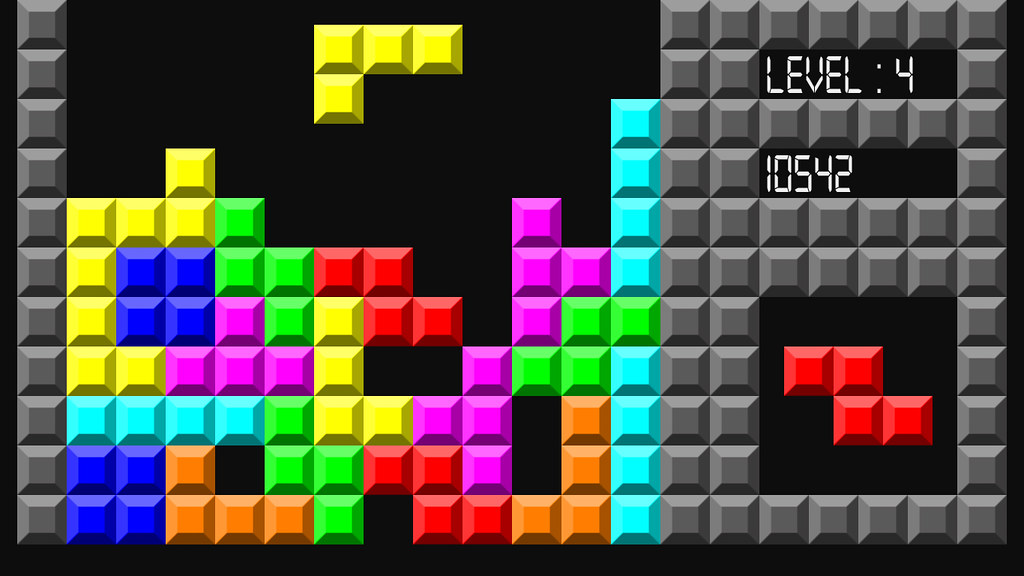
\includegraphics[width=\textwidth]{15538236401_a2eb533997_b.jpg}
    \end{subfigure}~%
    \begin{subfigure}{0.45\textwidth}
      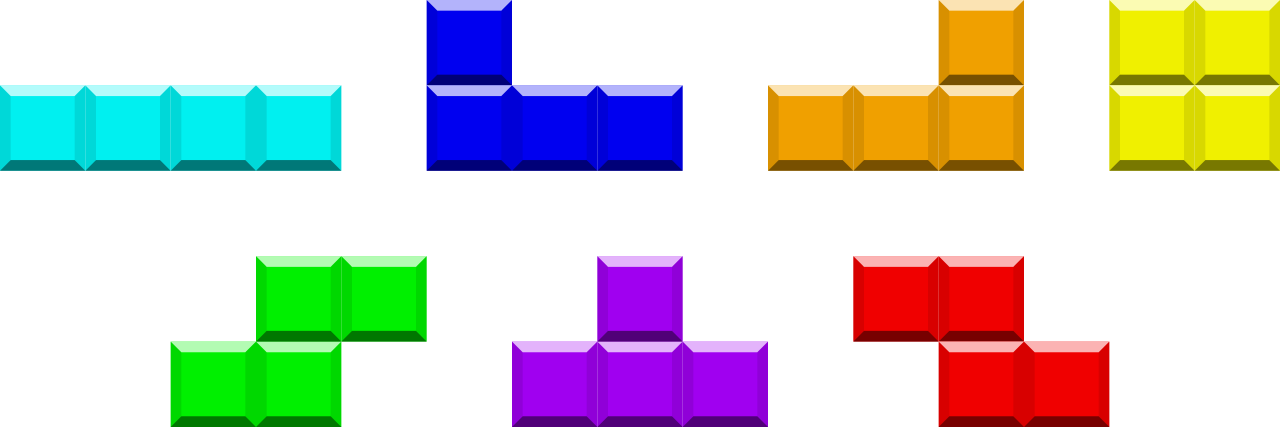
\includegraphics[width=\textwidth]{1280px-Tetrominoes_IJLO_STZ_Worlds.svg.png}
    \end{subfigure}
    \caption[asd]{A Tetris board shown to the left\footnotemark[1] and the seven available pieces show to the right\footnotemark[2]}
    \label{fig:tetris}
\end{figure}
\footnotetext[1]{\url{https://farm4.staticflickr.com/3938/15538236401_a2eb533997_b.jpg}}
\footnotetext[2]{\url{https://upload.wikimedia.org/wikipedia/commons/thumb/3/39/Tetrominoes_IJLO_STZ_Worlds.svg/1280px-Tetrominoes_IJLO_STZ_Worlds.svg.png}}

Tetris is a game first created by Alexey Pajitnov in 1989. The game consists of an initially empty grid (board) which is typically 20 rows by 10 columns big (as shown in figure~\ref{fig:tetris}). Each cell in the grid can be either filled or empty. One of seven different pieces (shown in figure~\ref{fig:tetris}), also called \emph{tetrimino}, spawn at the top of the board and are then placed by the player. The goal of the game is to get as high score as possible by forming full horizontal lines across the board. When one of these lines are created, it disappears and gives the player some amount of score, this will be referred to as ``clearing a line''. The game is played until a new piece can't be spawned, which happens when it intersects with another already placed piece when it spawns.

The game has been shown to always eventually terminate, i.e.\@ a game can not run forever\cite{TetrisLose}.
There are sequences of pieces that make the game terminate even if placed perfectly by an perfect player.

Our implementation of the game gives the score of 100 for each formed line and 5 for each piece placed.

\subsection{NEAT}
NEAT (NeuroEvolution of Augmenting Topologies) is a genetic algorithm developed by Kenneth Stanley in 2002\cite{NEAT}. The method is centered around evolving the topology (i.e. structure) and weights of neural networks rather than just optimizing the weights. Considerable time and effort can be saved using this method since no design has to be put into the topology of the network before training\cite{NEAT}. Instead, NEAT will start with a simple topology and make it more complex over time. When the initial topologies in the population are sufficiently different they will separate into distinct species and continue evolving separately, ensuring that newly created topologies have time to mature and optimize and is not removed prematurely\cite{NEATLearning}.

\subsection{Particle Swarm Optimization}
PSO (Particle Swarm Optimization) is an iterative optimization method developed by James Kennedy and Russel Eberhart~\cite{PSO}. The method uses a swarm of \textit{n} particles to explore a \textit{n}-dimensional search-space and iteratively proposes a solution. Each particle is a candidate solution and is associated with a position and a velocity. The movement of each particle is determined by its local best known position (the most optimal position the particle has visited) and the global best known position (the best position any particle in the swarm has visited). These two influences will move the swarm to the global minimum of the optimization function. Each particle is by some means interpreted as a solution, for example as a neural network of fixed structure by interpreting the position as weights.

\section{Related Work}

% Introduktion
There are a plethora of examples of algorithms being used to play Tetris as Sim{\'o}n Algorta et al.\@ summarizes in a paper\cite{TetrisML}.
One of which is a solution that Pierre Dellacherie\cite{pierre} made which extracts features from the Tetris board and weighs them against each other. 
This approach is explained in more detail in section~\ref{sec:features} and is the solution we had the most success with. The big difference is that Pierre hand-tuned all weights while we used machine learning to do it.

Jacob Schrum et al.\@\cite{comparingNEAT} compared a raw representation (similar to section~\ref{sec:naive}) to hand-designed features (similar to section~\ref{sec:features}) with NEAT and a variant of it called HyperNEAT to play Tetris.
Their choice of features were different from ours, they had 21 features based on Bertsekas\cite{bertsekas} while we had 6 other features based on Pierre\cite{pierre}.


% Tetris-AI https://github.com/fthomasmorel/Tetris-AI
%Tetris-AI is project by Thomas Morel where an AI was trained to play Tetris using genetic algorithms and the cross entropy method. 

% https://imake.ninja/el-tetris-an-improvement-on-pierre-dellacheries-algorithm/


\section{Approaches}\label{sec:approaches}

This section will explain the different approaches that was tried, what happened with each and what the reason for it working or not was.

\subsection{Naive Approach}\label{sec:naive}

\begin{wrapfigure}{r}{0.2\textwidth}
  \begin{center}
    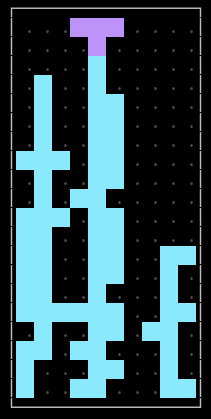
\includegraphics[width=0.18\textwidth]{naive.png}
  \end{center}
  \caption{}
  \label{fig:naive}
\end{wrapfigure}

The initial use of NEAT to play Tetris was naive. Each cell on the board was used as an input to the network, meaning there was 200 input nodes where a 1 represented a filled cell and a 0 an empty one. This input space was large, around $2^{10\cdot 20}$ different states, although many of which were invalid game states. There were six output nodes, representing six different actions: move left, move right, drop (move the piece all the way down), rotate left, rotate right and do nothing.

The game was played just like normal, no abstractions or simplifications. The flow was as follows:

\begin{enumerate}
    \item Feed the network with the board state.\label{first_step}
    \item Perform the action whose output node has the greatest numerical value.
    \item Move the piece one step down.
    \item Remove rows and/or spawn a new piece.
    \item Repeat from \ref{first_step} until Game Over\footnote{Popular term for stating that the game has finished}.
\end{enumerate}

This approach did not produce satisfactory result. The network learned to survive as long as possible by filling the board with three distinct towers (see figure~\ref{fig:naive}), it did not manage to clear any rows.

There are two big issues regarding this approach that makes learning more difficult, namely that the network has to find the current piece by itself and that there are too many steps before a piece lands.
The current piece is almost impossible to determine by just looking at the board. The network doesn't know how all different pieces look like or that they can be rotated, it has to somehow learn that by itself, which is a waste because that information can easily be provided as input to the network. It is also difficult for other reasons, for example, if the current piece is right next to a filled square, where does the current piece start and stop? That is impossible to tell and is probably why the network could not manage to build rows.

Having too many steps is also bad, because the network probably has a target location it wants to place the piece at right when it spawns and pushes it in the right direction. But it will be difficult to move it there because every step on the way also has to learn where the piece should land. It would be a lot better if the piece got placed in it is desired location immediately.

Another approach that does not have these problems is described in the following section.

\subsection{Naive Instant Place Approach}

To address the two problems from the previous section another approach was tested. Instead of playing the game with regular controls (move left, rotate right etc.) the game is played by dropping the piece on its desired location immediately. The network is given the current board state, the current piece to place and it outputs the location of where the piece should land and its orientation.

This approach uses a network with 207 inputs and 14 outputs. 200 of the inputs are the same as in the previous section, i.e.\@ each tile of the board. The seven new inputs tells the network which of the seven different pieces is the next piece to place. Ten of the outputs specifies which of the ten different columns the piece should be placed at and the last four specifies which orientation it should land with.

Immediately dropping a piece is not as flexible as using the regular controls. It is for example not possible to place a piece in a hole in a wall by pressing either left or right faster than the piece falls. We believe that there is a good possibility of training a good network without this rather special move.

A problem that still existed with this approach was the large input space, which mean that the exact same situation was not likely to happen more than once, hence it became hard to train the network. The network also never learned to fill up rows, but only to fill up the board just as the previous approach (figure~\ref{fig:naive}).

\subsubsection{More Complex Fitness Function}
To help the network understand how to eliminate rows were different fitness functions were derived. The fitness functions that were tried were to give more points the further down the piece lands, both linearly and exponentially, and give more points for each filled cell of the row that the piece lands on, also both linearly and exponentially. These fitness functions did not result in any improvements, the network still did not understand how to eliminates rows.

\subsection{Column Heights Approach}
One recurrent problem with the approaches mentioned in the previous sections was that the input space was to large. To address this issue the inputs to the network was redesigned, instead of taking each cell of the board as an input, only the heights of each column was given as input. The height of a column is defined as the distance between the bottom of the board and the cell closest to the top that is filled. This network has 17 inputs (10 for the columns and 7 for which piece) instead of previous 207 inputs. 

This approach has the main drawback of losing a lot of information. The network basically only sees how jagged the top of the board is, it does not see how many holes there are nor how filled each row is.
The performance of this approach was not good either and demonstrated the same behaviour as the previous approaches.

The input space can not really be reduced any further, so an overhaul of the general strategy was in order.

\subsection{Board Features Approach}\label{sec:features}

The main idea of this approach is that the network evaluate how good an action is rather than providing the action itself. This means that all possible actions should be considered by performing the action and then evaluating how good it was. The action with the highest score is the one actually executed. An action in this case is a position for a piece to be dropped at and a rotation for that piece. An outline of this new approach is as follows:

\begin{enumerate}
    \item Take a rotation and position.\label{bfa:start}
    \item Drop the piece and remove any complete rows.
    \item Extract \emph{features} from the board and feed them to a neural network that will output a score.
    \item Reset the board.
    \item Repeat from \ref{bfa:start} until all possible rotations and positions have been tested.
    \item Drop the piece a final time at the position and rotation with the highest score.
\end{enumerate}

A \emph{feature} is a relevant characteristic used to evaluate a board state. These features were inspired by Pierre Dellacherie\cite{TetrisML} and are defined as follows:

\begin{description}
    \item[Rows:] the number of eliminated rows the dropped piece eliminated, a number between zero and four.
    \item[Landing height:] the height at which the dropped piece will land at after all rows have been eliminated, the height is calculated from the piece's top.
    \item[Holes:] the number of inaccessible cells, which is defined as the number of empty cells that has at least one filled cell above it.
    \item[Wells:] the number of cells that has the cells immediately to the left and right of it filled and cells above it is not filled.
    \item[Column transitions:] the amount of transitions within all columns, where a transition is a cell that has a neighbour of the other type (filled or not filled).
    \item[Row transitions:] the amount of transitions within all rows, where a transition is defined the same as with column transitions.
\end{description}

\begin{figure}[t]
    \centering
    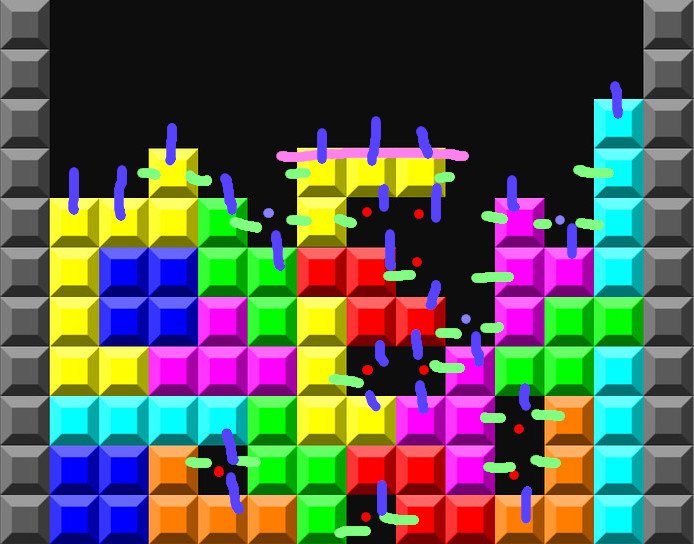
\includegraphics[width=0.7\textwidth]{tetris_annotated.jpg}
    \caption{Annotated board state from dropping the yellow floating piece from figure~\ref{fig:tetris} showing example of all features from section~\ref{sec:features}. The red dots are the holes, the blue dots are the wells, the green lines are row transitions, the blue lines are column transitions and the purple line marks the landing height. There were no lines eliminated.}
    \label{fig:tetris:anot}
\end{figure}

The network is trained to evaluate all these features against each other and provides a score based on these features. The network has then six inputs and one output.
This approach turned out to be the most successful of them all, managing to get scores in the millions, i.e.\@ hundreds of thousands of lines cleared.
A picture of the best network produced (both overall and with this approach) is shown in figure~\ref{fig:graph}.

The importance and role of each feature is explored in the next section.

\subsubsection{Feature Analysis}\label{sec:features:anal}

\begin{figure}[ht]
    \centering
    \begin{tikzpicture}
    \begin{axis}[
      grid=major,
      width=\textwidth,
      ylabel={Fitness},
      xlabel={Generations},
      no markers,
      every axis plot/.append style={thick, line join=round},
      cycle list name=color list non retard,
      enlargelimits=false,
      legend style={cells={anchor=west}, legend pos=north east},
      xmax=30
    ]
\addplot coordinates {(1,10405.0) (2,11540.0) (3,23495.0) (4,37070.0) (5,30075.0) (6,38310.0) (7,47305.0) (8,37745.0) (9,32325.0) (10,41905.0) (11,40625.0) (12,61460.0) (13,23445.0) (14,25455.0) (15,22045.0) (16,28490.0) (17,40775.0) (18,24325.0) (19,34470.0) (20,39550.0) (21,31760.0) (22,44250.0) (23,39765.0) (24,45380.0) (25,70590.0) (26,32870.0) (27,34260.0) (28,40195.0) (29,23340.0) (30,23545.0) (31,24225.0) (32,25340.0) (33,67875.0) (34,32120.0) (35,47745.0) (36,25035.0) (37,42425.0) (38,28285.0) (39,23285.0) (40,58410.0) (41,28815.0) (42,31885.0) (43,32790.0) (44,27165.0) (45,24015.0) (46,38860.0) (47,22900.0) (48,48650.0) (49,46500.0) (50,47715.0)}; \addlegendentry{hrl} \label{fig:plot4:hrl}
%\addplot coordinates {(1,1055.0) (2,890.0) (3,505.0) (4,2455.0) (5,425.0) (6,1410.0) (7,1075.0) (8,1085.0) (9,2460.0) (10,780.0) (11,1530.0) (12,1520.0) (13,655.0) (14,1090.0) (15,1880.0) (16,865.0) (17,1080.0) (18,1080.0) (19,1120.0) (20,2330.0) (21,1100.0) (22,875.0) (23,4575.0) (24,855.0) (25,1090.0) (26,1405.0) (27,860.0) (28,1080.0) (29,1315.0) (30,640.0) (31,770.0) (32,1765.0) (33,625.0) (34,745.0) (35,1305.0) (36,1745.0) (37,645.0) (38,745.0) (39,1455.0) (40,750.0) (41,1565.0) (42,990.0) (43,640.0) (44,525.0) (45,965.0) (46,820.0) (47,1185.0) (48,2435.0) (49,1070.0) (50,1300.0)}; \addlegendentry{hr} \label{fig:plot4:hr}
\addplot coordinates {(1,2070.0) (2,2740.0) (3,2970.0) (4,2855.0) (5,2305.0) (6,2850.0) (7,2630.0) (8,5110.0) (9,2980.0) (10,2525.0) (11,2865.0) (12,3655.0) (13,2865.0) (14,3085.0) (15,3085.0) (16,2195.0) (17,2640.0) (18,2755.0) (19,2630.0) (20,3200.0) (21,3190.0) (22,2865.0) (23,2415.0) (24,2855.0) (25,2745.0) (26,3310.0) (27,3205.0) (28,3305.0) (29,3080.0) (30,2745.0)}; \addlegendentry{rl} \label{fig:plot4:rl}
    \end{axis}
    \end{tikzpicture}
    \caption{The maximum fitness when training over 30 generations.
    Plot~\ref{fig:plot4:rl} uses \textbf{rows} and \textbf{landing height} while
    %plot~\ref{fig:plot4:hr} uses \textbf{holes} and \textbf{rows}, finally
    plot~\ref{fig:plot4:hrl} uses \textbf{rows}, \textbf{landing height} and \textbf{holes}.}
    \label{fig:plot4}
\end{figure}
\begin{figure}[ht]
    \centering
    \begin{tikzpicture}
    \begin{axis}[
      grid=major,
      width=\textwidth,
      ylabel={Fitness},
      xlabel={Generations},
      no markers,
      every axis plot/.append style={thick, line join=round},
      cycle list name=color list non retard,
      enlargelimits=false,
      xmax=35,
      legend style={cells={anchor=west}, legend pos=north east}
    ]
\addplot coordinates {(1,270360.0) (2,414035.0) (3,320095.0) (4,774135.0) (5,346090.0) (6,716680.0) (7,356770.0) (8,361690.0) (9,369160.0) (10,878560.0) (11,314605.0) (12,880230.0) (13,1000040.0)}; \addlegendentry{-h} \label{fig:plot2:h}
\addplot coordinates {(1,5350.0) (2,17160.0) (3,135370.0) (4,1000055.0)}; \addlegendentry{-ct} \label{fig:plot2:ct}
\addplot coordinates {(1,96260.0) (2,161825.0) (3,1000050.0)}; \addlegendentry{-r} \label{fig:plot2:r}
\addplot coordinates {(1,16225.0) (2,99120.0) (3,813190.0) (4,1000065.0)}; \addlegendentry{-rt} \label{fig:plot2:rt}
\addplot coordinates {(1,104335.0) (2,155280.0) (3,284435.0) (4,373875.0) (5,250235.0) (6,720590.0) (7,644225.0) (8,360045.0) (9,360490.0) (10,189480.0) (11,177575.0) (12,463305.0) (13,211900.0) (14,404140.0) (15,429805.0) (16,756825.0) (17,669290.0) (18,367600.0) (19,508660.0) (20,840530.0) (21,659180.0) (22,341045.0) (23,362385.0) (24,412370.0) (25,239455.0) (26,324830.0) (27,1000040.0)}; \addlegendentry{-w} \label{fig:plot2:w}
\addplot coordinates {(1,44560.0) (2,66845.0) (3,50745.0) (4,178750.0) (5,120725.0) (6,91240.0) (7,58945.0) (8,104560.0) (9,98155.0) (10,118915.0) (11,71350.0) (12,185420.0) (13,122975.0) (14,70585.0) (15,318355.0) (16,358335.0) (17,411220.0) (18,153335.0) (19,191720.0) (20,214570.0) (21,166700.0) (22,121665.0) (23,133640.0) (24,136220.0) (25,179255.0) (26,144560.0) (27,184620.0) (28,142950.0) (29,185760.0) (30,381715.0) (31,207010.0) (32,103395.0) (33,186345.0) (34,183910.0) (35,406695.0) (36,306360.0) (37,237090.0) (38,651185.0) (39,424930.0) (40,224090.0) (41,287380.0) (42,178925.0) (43,316805.0) (44,278200.0) (45,310080.0) (46,333260.0) (47,277895.0) (48,229925.0) (49,261870.0) (50,157990.0)}; \addlegendentry{-lh} \label{fig:plot2:lh}
    \end{axis}
    \end{tikzpicture}
    \caption{The maximum fitness when training with a score limit (fitness) of one million over 35 generations. Plot~\ref{fig:plot2:h} has all features enabled except \textbf{holes}, plot~\ref{fig:plot2:ct} has all features except \textbf{column transitions}, plot~\ref{fig:plot2:r} has all features except \textbf{rows}, plot~\ref{fig:plot2:rt} has all features except \textbf{row transitions}, plot~\ref{fig:plot2:w} has all features except \textbf{wells} and finally plot~\ref{fig:plot2:lh} has all features except \textbf{landing height}.}
    \label{fig:plot2}
\end{figure}
\begin{figure}[ht]
    \centering
    \begin{tikzpicture}
    \begin{axis}[
      grid=major,
      width=\textwidth,
      ylabel={Fitness},
      xlabel={Generations},
      no markers,
      every axis plot/.append style={thick, line join=round},
      cycle list name=color list non retard,
      enlargelimits=false,
      legend style={cells={anchor=west}, legend pos=south east}
    ]
\addplot coordinates {(1,33245.0) (2,633415.0) (3,414715.0) (4,1658855.0) (5,3743040.0) (6,5000075.0)}; \addlegendentry{all} \label{fig:plot3:all}
\addplot coordinates {(1,48520.0) (2,398270.0) (3,577370.0) (4,154250.0) (5,238080.0) (6,607195.0) (7,1257105.0) (8,1036040.0) (9,2636035.0) (10,811625.0) (11,920760.0) (12,5000085.0)}; \addlegendentry{-r} \label{fig:plot3:r}
\addplot coordinates {(1,145960.0) (2,155195.0) (3,114885.0) (4,117605.0) (5,164060.0) (6,455225.0) (7,952130.0) (8,815655.0) (9,665150.0) (10,1857635.0) (11,2108865.0) (12,1046420.0) (13,973160.0) (14,2129675.0) (15,1531840.0) (16,2439370.0) (17,5000000.0)}; \addlegendentry{-ct, -rt} \label{fig:plot3:ctrt}
\addplot coordinates {(1,41545.0) (2,262505.0) (3,980585.0) (4,196580.0) (5,220415.0) (6,291850.0) (7,496515.0) (8,1012420.0) (9,1292440.0) (10,1471755.0) (11,2631300.0) (12,1160355.0) (13,3381975.0) (14,1467265.0) (15,1619680.0) (16,1182045.0) (17,5000100.0)}; \addlegendentry{-rt} \label{fig:plot3:rt}
\addplot coordinates {(1,12105.0) (2,643900.0) (3,874720.0) (4,740170.0) (5,245525.0) (6,389510.0) (7,945050.0) (8,406845.0) (9,260430.0) (10,1081170.0) (11,256970.0) (12,2447375.0) (13,1266210.0) (14,1253135.0) (15,453085.0) (16,2008175.0) (17,3167490.0) (18,3185265.0) (19,630850.0) (20,2454445.0) (21,4385260.0) (22,2298925.0) (23,2317550.0) (24,5000075.0)}; \addlegendentry{-ct} \label{fig:plot3:ct}
    \end{axis}
    \end{tikzpicture}
    \caption{The maximum fitness when training with a score limit (fitness) of 5 million over 24 generations. Plot~\ref{fig:plot3:all} has all features enabled, plot~\ref{fig:plot3:r} has all features except \textbf{rows}, plot~\ref{fig:plot3:ctrt} has all features except \textbf{column transitions} and \textbf{row transitions}, plot~\ref{fig:plot3:rt} has all features except \textbf{row transitions} and finally plot~\ref{fig:plot3:ct} has all features except \textbf{column transitions}. }
    \label{fig:plot3}
\end{figure}

The general goal of Tetris is to eliminate as many rows as possible (that is the main way to get score) and to not fill the board to the top, because then the game is over and the ability to get more score is gone.
This naturally justifies the existence of the \textbf{rows} and \textbf{landing height} features. The network should prefer actions that eliminates many rows while trying to place the pieces as close to the bottom as possible. Plot~\ref{fig:plot4:rl} in figure~\ref{fig:plot4} shows that this is not enough, there is an aspect missing, namely the number of holes. Minimizing the number of holes is important because a hole is just dead space, it can not be reached by a piece and hence can not form a full row. Plot~\ref{fig:plot4:hrl} in figure~\ref{fig:plot4} shows that the introduction of the \textbf{holes} feature dramatically improves things.

Figure~\ref{fig:plot2} illustrates the importance of each feature by showing the results of training sessions with all features except for one, one session for each omitted feature. Plot~\ref{fig:plot2:lh} and plot~\ref{fig:plot2:h} perform worse than the other ones, which makes sense because the landing height and the number of holes are important, as already discussed. This figure shows another feature that seems important, namely \textbf{wells} shown on plot~\ref{fig:plot2:w}.
Wells are not desirable because they can be hard to fill without leaving holes. A well with deep three or more can only be filled with a 1x4 piece, which is only one out of seven available pieces.
The other plots in the same figure reached a score of one million quickly, indicating that \textbf{rows}, \textbf{row transitions} and \textbf{column transitions} are not that important. But  maybe they are, they may just grow quickly in the beginning but are not able to reach a high score in the long run.

Figure~\ref{fig:plot3} shows these three and some more up to a score of five million instead of one million. Having all features enabled (\ref{fig:plot3:all}) gives the best result out of everything, showing that all these six features are needed. The excluded \textbf{rows} runs from figure~\ref{fig:plot2} did indeed not perform as well in the long run as seen in figure~\ref{fig:plot4}.

Both transition features plays the role of making sure that all pieces are placed compactly against each other, making sure that there are few gaps. Having pieces placed without gaps is good because it makes it easier for future pieces to be placed without creating holes. Figure~\ref{fig:plot3} shows that training up to five million is a lot slower without any transition feature, so they are important.

% kanske försöka förklara skillnaden mellan holes och ct

\section{Comparison to PSO}

\begin{figure}[t]
    \centering
    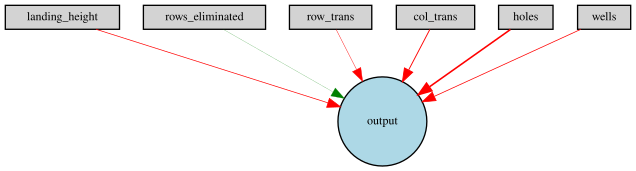
\includegraphics[width=0.8\textwidth]{graph0.png}
    \caption[asd]{Illustration of a network that produced a fitness of 55 million using the approach described in section~\ref{sec:features}. The rectangles are the input nodes, the blue is the output node and the arrows are the weights where a red color is a negative weight and a green color is a positive weight. The thickness of each arrow illustrates how big the value of the weight is.
    
    \medskip
    \centering
    \begin{tabular}{lr@{.}l}
        Wells & -2 & 2325745006784596\\
        Holes & -5 & 468481414786788\\
        Column Transitions & -2 & 9407012203149034\\
        Row Transitions & -1 & 066752716475175\\
        Rows Eliminated & 0 & 21727304852256102\\
        Landing Height & -2 & 078277000532176
    \end{tabular}
    }
    \label{fig:graph}
\end{figure}

The successful approaches from section~\ref{sec:approaches} all converged to the same network structure, an example of which can be seen in figure~\ref{fig:graph}. The structure consists of one output node with a linear activation function, no hidden nodes and all input nodes connected to the output node, meaning that the output of the network is a simple weighted sum of all inputs.

One advantage of using NEAT is the natural exploration of different network structures. Therefore, if NEAT consistently produces the same structure then perhaps NEAT is not the most suitable method for this problem. PSO can be used to optimize a neural network with a fixed structure by searching a \textit{n}-dimensional space where each dimension represents a weight or a bias. In this case a seven dimensional method was used: one weight for each of the six inputs and one bias. PSO performed well in just a few iterations, oftentimes reaching a fitness of around 5 million in the first few iterations.

\section{Conclusions and Future Work}
%Summarize your contribution
%Conclusions from the results
%Implications for the future

Here we present various conclusions and potential future work or explorations that could be interesting to find answers to.

\subsection{Approach conclusions}
% säga  hur bra våran är jämfört med alla andras??
We managed to get a working Tetris AI that scored in the millions with our rule set. The best score was 55 million, which is about 500000 cleared lines.
Our AI can most likely score higher 

We can conclude from our different approaches that it is beneficial to make the work of the network as simple as possible.
Having the network see every cell as input, as explained in section~\ref{sec:naive}, was not good at all. The input space to the network was too big and the network had to make a complex decision.
It ended up filling the board as much as possible instead of actually building rows.
The key for fixing this was to offload some work of the network by having the network evaluate moves and perform the best one instead of directly deciding the move to make.
That is what we did with the feature extraction approach explained in section~\ref{sec:features}.
Simplifying and abstracting helped for Tetris and is most likely a good approach for other machine learning related problems as well.

All the features we used in the best and final approach, i.e.\@ feature extraction (section~\ref{sec:features}), each contributed to something as shown in section~\ref{sec:features:anal}.
The results in that section is not that reliable because most of the runs were only run once. Tetris is stochastic, sometimes when training the network it is not able to get high scores at all and sometimes it reaches very high scores on the second generation. But even though we can not draw reliable conclusions with absolute confidence our test runs are at least somewhat representative of their actual behaviour. During the training sessions there were also score limits to reduce computing time, which further reduces the reliability of the test results.

Jacob Schrum et al.\@\cite{comparingNEAT}, whom did a similar study, got the same results i.e.\@ raw input from the board did not work well and feature extraction worked better.

\subsection{Approach future work}
All of the approaches presented in this paper only looked at one piece at a time, but to consider two or more pieces at a time should be able to give better results.
This can easily be done in with the features approach (section~\ref{sec:features}) by placing two pieces after each other before extracting all features. This will lead to many more possibilities to evaluate, which will lead to the question of if it is worth it? The potential for high scores might not be that much higher than the single piece approach, not making the extra computations worth it.

\subsection{Training algorithm conclusions}

The PSO algorithm is likely better suited for this problem due to its faster learning speed. This is in large part because PSO does not explore different network structures, so it can start optimizing the weights straight away and can propose a good solution early. 
However, for the PSO algorithm to work the structure of the network needs to be defined beforehand, which was provided by NEAT. This makes it difficult to conclude that one method is strictly better than the other, but in situations where the structure of the network is provided, PSO would be preferred over NEAT.

\bibliographystyle{plain}
\bibliography{referenser} 

\end{document}


%Dagbok:
%%Dag 1.
%Första försök: 200input 4output, varje ruta in, knapptryck ut
%  Det funkar nog inte så bra för att det är fler steg att göra (och därmed lära sig) för att plonka ner en bit. Är nog bättre att plonka ned på en gång, vi förlorar flexibilitet och coolhet dock.

%Andra försök: Ändra output till position (14outputs)
%  Den körde mkt snabbare, ingen förbättring dock, kanske för många inputs. Den verkar lära sig att fylla brädet, inte göra rader, kanske behöver bättre fittness.

%Tredje försök: Ändrat fitness:
%    Poäng för block och rad
%    Poäng för bara rad
%    Poäng för hur iflyllda raderna är
%    och massor av kombinationer utav e^x o grejer för att ge mer poäng för block i botten i ett försök att få den att inte bygga torn.
    
%Fail: Glömde informera nätverket om vilket block den hade. Den lärde sig inte när det blev fixat ändå :(

%%Dag 2.
%glömde ge rotation också, men blev ingen skillnad för det.

%tes: för många inputs. Spara höjderna istället. Att spara varje block tjänar inget till då vi droppar bitarna på en gång.
%  Det blev mkt snabbare! Men den lär sig fortfarande inte.

%tes: testa att evaluera på fler spel än ett för att ge varje individ en ärligare chans.
%  blev inte så mkt bättre

%tes: ge varje individ i en generation samma seed så att de får samma block så att det blir jämnare.
%  Slutade med att alla fastnade på att göra exakt samma sak varje gång, så tog bort denna.

%efter att ha tränat i 6500-ish rundor så får den bara 200-ish, alltså två rader

% Discussion about a somewhat fixed topology, seems to yield just one node

%%Dag 3.
%att använda höjderna som input tar bort viktig info, som typ hur många hål det finns.
%kopierade https://imake.ninja/el-tetris-an-improvement-on-pierre-dellacheries-algorithm/

%tes: inputrymden är för stor för NEAT! Så om vi minskar den genom att själva extrahera viktiga egenskaper från brädet och ger det som input istället.
% Det blev bättre, nu har vi ett snitt på ~3 rader.
% Det blev ännu bättre när den kunde mutera till en linjär activation function.
% En bild på nätverket visar att den väljer att ignorera vissa inputs, men vi vill ju att den alltid ska bry sig om alla inputs nu när vi har sagt åt den specifikt vad den ska titta på. Vi kanske måste byta till swarm, eller åtminstone ha en fixerad nätverksstruktur.

% Swarm
% tes: det verkar son att strukturen på nätverket efter NEAT är bara en nod, därför kanske swarm passa bättre?
% resultat: Swarm fick mycket bra fitness efter bara några iterationer

% tes: sigmoid suger för att input-värdena inte är normaliserade.
% verkar stämma, blev galet mycket bättre, men inte lika bra som linjär. Hade dock tanh istället för sigmoid, ish samma sak.
